\section{Force}

\begin{multicols}{2}

\section*{Concept of Force}


\subsection{Examples of Forces}
\begin{center}
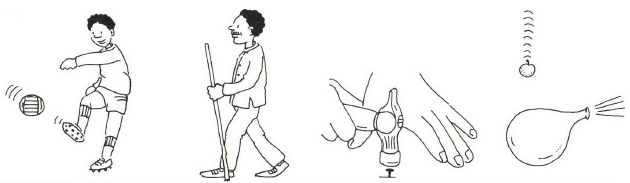
\includegraphics[width=0.4\textwidth]{./img/vso/forces-ex.png}
\end{center}

\subsection{Making a Spring Balance}

\begin{center}
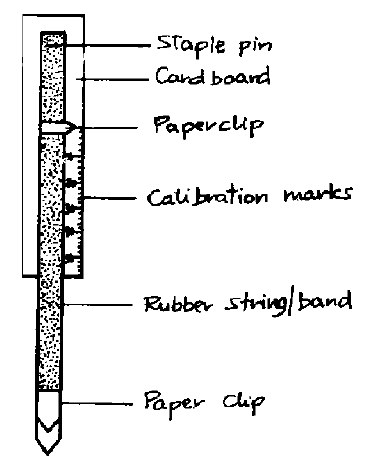
\includegraphics[width=0.4\textwidth]{./img/source/spring-balance.png}
\end{center}

\begin{description*}
%\item[Subtopic:]{Concept of Force}
%\item[Shika Rating:]{4}
\item[Materials:]{Cardboard, strong rubber band, staple pin, 2 paper clips, \nameref{sec:masses}*}
\item[Setup:]{Take a strip of cardboard or wood and fix a strong rubber band to it using a staple pin. (The stronger the rubber band, the larger the force you can measure.) Attach one paper clip as a pointer as shown in the figure. Then fix another as a hook at the bottom end of the rubber band.}
\item[Procedure:]{Calibrate the balance in \emph{Newtons} using either a standard set of \nameref{sec:masses} or another spring balance. A mass of 10 g has a weight of 0.1 N; a mass of 100 g has a weight of 1 N, etc. Draw marks accordingly on the scale of the balance.}
\item[Hazards:]{Never apply such a large force that the pointer does not return to the zero mark when the force ceases.}
%\item[Questions:]{}
%\item[Theory:]{}
\item[Applications:]{Use the spring balance to measure the weight of small objects or the force of pulling an object along a table.}
%\item[Notes:]{}
\end{description*}

%==================================================================================================%

\section*{Effects of Forces}
Forces can have a variety of effects on objects, including \emph{stretching}, \emph{compression} (or \emph{restoring}), \emph{attraction}, \emph{repulsion}, \emph{torsion}, \emph{friction}, \emph{viscosity} and \emph{air resistance}. These effects are seen all around us in our daily lives.


\subsection{Observing Effects of Forces}
\begin{description*}
%\item[Subtopic:]{}
\item[Materials:]{Rubber bands, springs, magnets, ruler, honey, water, paper}
%\item[Setup:]{}
\item[Procedure:]{Have students investigate different effects of forces using common materials.}
%\item[Hazards:]{}
%\item[Questions:]{}
\item[Observations:]{Rubber bands and springs stretch when pulled and then restore their shape. Magnets attract and repel each other. A ruler can be twisted under torsion. Rubbing hands together produces heat from friction. Honey pours more slowly than water due to a higher viscosity. A sheet of paper falls to the ground slowly because of air resistance.}
%\item[Theory:]{}
\item[Applications:]{Brainstorm various applications of the effects of forces with the class.}
%\item[Notes:]{}
\end{description*}

\subsection{Presence of Gravity}
\begin{description*}
%\item[Subtopic:]{}
\item[Materials:]{Pen, ruler, sheet of paper, book (same size as paper)}
%\item[Setup:]{}
\item[Procedure:]{Drop the pen and ruler side by side from shoulder height. Repeat with a pen and sheet of paper. Then place the paper on top of a book and drop side by side with a regular sheet of paper. Bunch the paper into a tight ball and drop it again with the book.}
%\item[Hazards:]{}
\item[Questions:]{Which objects fell at the same rate? Which ones fell more slowly?}
\item[Observations:]{All objects, with the exception of paper and other light, wide objects, fall at exactly the same rate.}
\item[Theory:]{Gravity pulls on all objects on earth the same.  The paper falls slowly because the paper is more affected by air resistance. All objects are affected by air resistance, but it is most obvious with objects that have a small weight with a large surface area. Placing a book under the paper reduces air resistance by blocking all of the air which would normally push against the paper. Thus they fall at the same rate.  When the paper is bunched into a ball, the mass stays the same but the air resistance is greatly reduced so it should fall at the same rate as the book.}
%\item[Applications:]{}
%\item[Notes:]{}
\end{description*}

\subsection{Parachutes}

\begin{center}
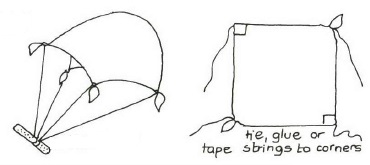
\includegraphics[width=0.4\textwidth]{./img/vso/parachute.png}
\end{center}

\begin{description*}
%\item[Subtopic:]{}
\item[Materials:]{Paper/newspaper/plastic bags, string, paper clips}
\item[Setup:]{Tie pieces of string (about 30 cm) to each corner of the paper/bag. Join the four strings together and attach a paper clip or other small weight.}
\item[Procedure:]{Drop the parachute side by side with a normal paper clip.}
%\item[Hazards:]{}
\item[Questions:]{Which one reaches the ground first? If the paper clip were a person, which one would arrive safely to the ground? Does a person using a parachute want to make it as large as possible or as small as possible?}
\item[Observations:]{The parachute falls more slowly because there is a larger space for air to enter and counteract the force of gravity pulling it to the ground.}
%\item[Theory:]{}
\item[Applications:]{Skydivers, military personnel, air-dropped aid packages}
\item[Notes:]{Poke a small hole in the top of the parachute and ask students what will happen.}
\end{description*}

\subsection{Helicopters}

\begin{center}
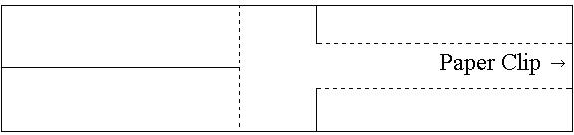
\includegraphics[width=0.4\textwidth]{./img/helicopter-1.png}
\end{center}

\begin{center}
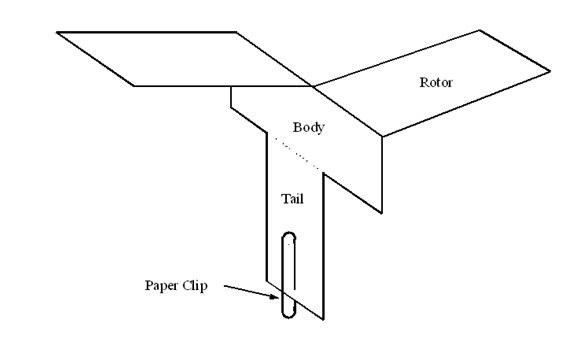
\includegraphics[width=0.4\textwidth]{./img/helicopter-2.png}
\end{center}

\begin{description*}
%\item[Subtopic:]{}
\item[Materials:]{Paper, scissors, paper clip}
%\item[Setup:]{}
\item[Procedure:]{Copy the following design onto a piece of paper. Cut along the solid lines and fold along the dotted lines, attaching the paper clip to the bottom. Drop the helicopter with the paperclip down and watch it spin!}
%\item[Hazards:]{}
\item[Questions:]{Does the helicopter spin more if you add more paper clips? If you change the size/number of wings?}
\item[Observations:]{Adding more paper clips causes the helicopter to spin faster. Increasing the surface area of the wings also increases the rate of spin.}
\item[Theory:]{The helicopter spins because the force of air resistance pushing up on the wings creates a moment about the vertical axis of rotation. Increasing the force of air resistance thus increases this moment and hence the helicopter spins faster.}
%\item[Applications:]{}
%\item[Notes:]{}
\end{description*}


\end{multicols}

\pagebreak